
\documentclass[sigconf]{acmart}

\setcopyright{none}
\settopmatter{printacmref=false}
\renewcommand\footnotetextcopyrightpermission[1]{}
\usepackage{pdfpages}
\usepackage{tabularx}
\usepackage{float}
%%
%% end of the preamble, start of the body of the document source.
\begin{document}
\pagestyle{empty}
%%
%% The "title" command has an optional parameter,
%% allowing the author to define a "short title" to be used in page headers.
\title{\textbf{OrcaLink: Modeling Potential Social Ties in Southern Resident Killer Whales}}

%%
%% The "author" command and its associated commands are used to define
%% the authors and their affiliations.
%% Of note is the shared affiliation of the first two authors, and the
%% "authornote" and "authornotemark" commands
%% used to denote shared contribution to the research.

\author{Aung Htut}
\email{amhtut@uvic.ca}
\affiliation{%
  \institution{University of Victoria}
   \city{Victoria}
   \country{Canada}
}
\author{Bowen Zhang}
\email{bowenzhang1@uvic.ca}
\affiliation{%
  \institution{University of Victoria}
   \city{Victoria}
   \country{Canada}
}

%%
%% The abstract is a short summary of the work to be presented in the
%% article.
\begin{abstract}
Southern Resident killer whales (SRKWs) have multiple types of relationships, including pod membership, matrilineal kinship, and social associations. Genealogical and relationship information must be considered together with sighting and encounter information to comprehensively query familial and social relationships among individuals. This paper reviews how existing sources represent these records and compares their strengths and limitations. Based on this review, OrcaLink proposes a draft data model that integrates relationship and sighting information to explore observed associations and potential association candidates based on shared associations and kinship. The project repository is available at \url{https://github.com/CSC501-OrcaLink/orcalink}.
\end{abstract}

\maketitle

\begin{table*}[!t]
\caption{Comparison of the records reviewed for OrcaLink.}
\label{tab:source-comparison}
\small
\setlength{\tabcolsep}{4pt}
\renewcommand{\arraystretch}{1.15}

\begin{tabularx}{\textwidth}{
  @{}>{\raggedright\arraybackslash}p{1.5cm}
  *{5}{>{\raggedright\arraybackslash}X}@{}
}

\toprule
\textbf{Source} &
\textbf{Main purpose} &
\textbf{Key entities or records} &
\textbf{Key relationships} &
\textbf{Strengths} &
\textbf{Limitations} \\
\midrule

CWR public records \cite{cwrOrcaID} &
Identify whales, describe family structure, and document encounters &
Whales, pods, matrilines, encounters &
Family relationships, pod membership, and encounter participation &
Connect individual identity and family information across records &
Public records alone do not provide a complete structured encounter dataset for our comparison \\
\midrule

Dryad dataset \cite{thompson2026dryad} &
Organize observations for J-pod movement analysis &
Whale IDs, sighting IDs, timestamps, coordinates, lifespan records &
Whale records linked through shared sighting IDs &
Supports recorded co-sighting queries &
Some IDs are assigned based on group reports or are missing; timestamps and coordinates are shifted \\
\midrule

Whale Museum dataset \cite{whalemuseum_dataset} &
Maintain historical sighting records &
Reports, reported groups, dates, locations, sources &
Reported groups linked to sightings &
Supports group-presence queries across time and locations &
Supplied records do not identify individual whales \\
\bottomrule
\end{tabularx}
\end{table*}

\section{Introduction}

Southern Resident killer whales (SRKWs) generally travel in matrilineal family groups but also form social associations \cite{ellis2017}. Encounter and photo-identification records have been collected since 1976 \cite{cwrhistory}. Individual records describe whales' identities, demographic information, and matrilineal relationships \cite{orcaConservancy}, while sighting records identify individuals observed together, along with dates and locations \cite{thompson2026dryad}. However, some individual identifiers in the Dryad sighting data are assigned based on reports of an entire pod or matriline rather than individually confirmed observations \cite{thompson2026dryad}.

Family membership and observed associations represent different types of relationships. Although previous studies have investigated demographic and social association data \cite{ellis2017}, examining individual records alone makes it difficult to jointly query kinship, repeated co-sightings, and indirect connections across multiple encounters. For OrcaLink, recorded co-sightings will be treated as evidence of shared observations rather than confirmation of a close social relationship. OrcaLink aims to integrate these relationships into a data model that supports queries about both direct and indirect associations among individuals while retaining their sources and identification information.

This paper reviews the history of individual identification and encounter recording, compares existing representations, and uses their strengths and limitations to guide OrcaLink's draft ER model.

\section{History}

Individual photo-identification developed in the 1970s through Michael Bigg's work, using photographs of dorsal fins and saddle patches to distinguish whales \cite{cwrOrcaID}. CWR's first documented encounter was on April 8, 1976, when K and L pods were observed near Dungeness Spit. The encounter was recorded in a handwritten logbook and through film photographs \cite{cwrFirstEncounter}. Its first J-pod encounter followed on April 16, 1976 \cite{cwrhistory}. These are the first encounters documented by CWR, rather than the first-ever sightings of these whales. Early film photographs were developed and reviewed to identify individuals, while current identification uses digital photographs examined on computers \cite{cwrOrcaID}.

The Whale Hotline public sighting network started in spring 1976, allowing members of the public to report orca sightings in Washington State by telephone. Today, reports can be submitted online, by phone, or by email. The Whale Museum gathers these reports, and staff work to confirm sightings before entering them into the database \cite{whaleHotline}. The dataset provided for this project also contains earlier records, with the earliest dated row being December 6, 1948. However, the row does not explain how the original observation was recorded \cite{whalemuseum_dataset}.

Recording methods have developed from handwritten logs, film photographs, and telephone reports to digital images and database records. OrcaLink must preserve their sources and distinguish group reports from individually identified sightings.

\section{Hierarchy}

Figure~\ref{fig:hierarchy} groups the reviewed representations by their main purpose. 

\begin{figure}[H]
    \centering
    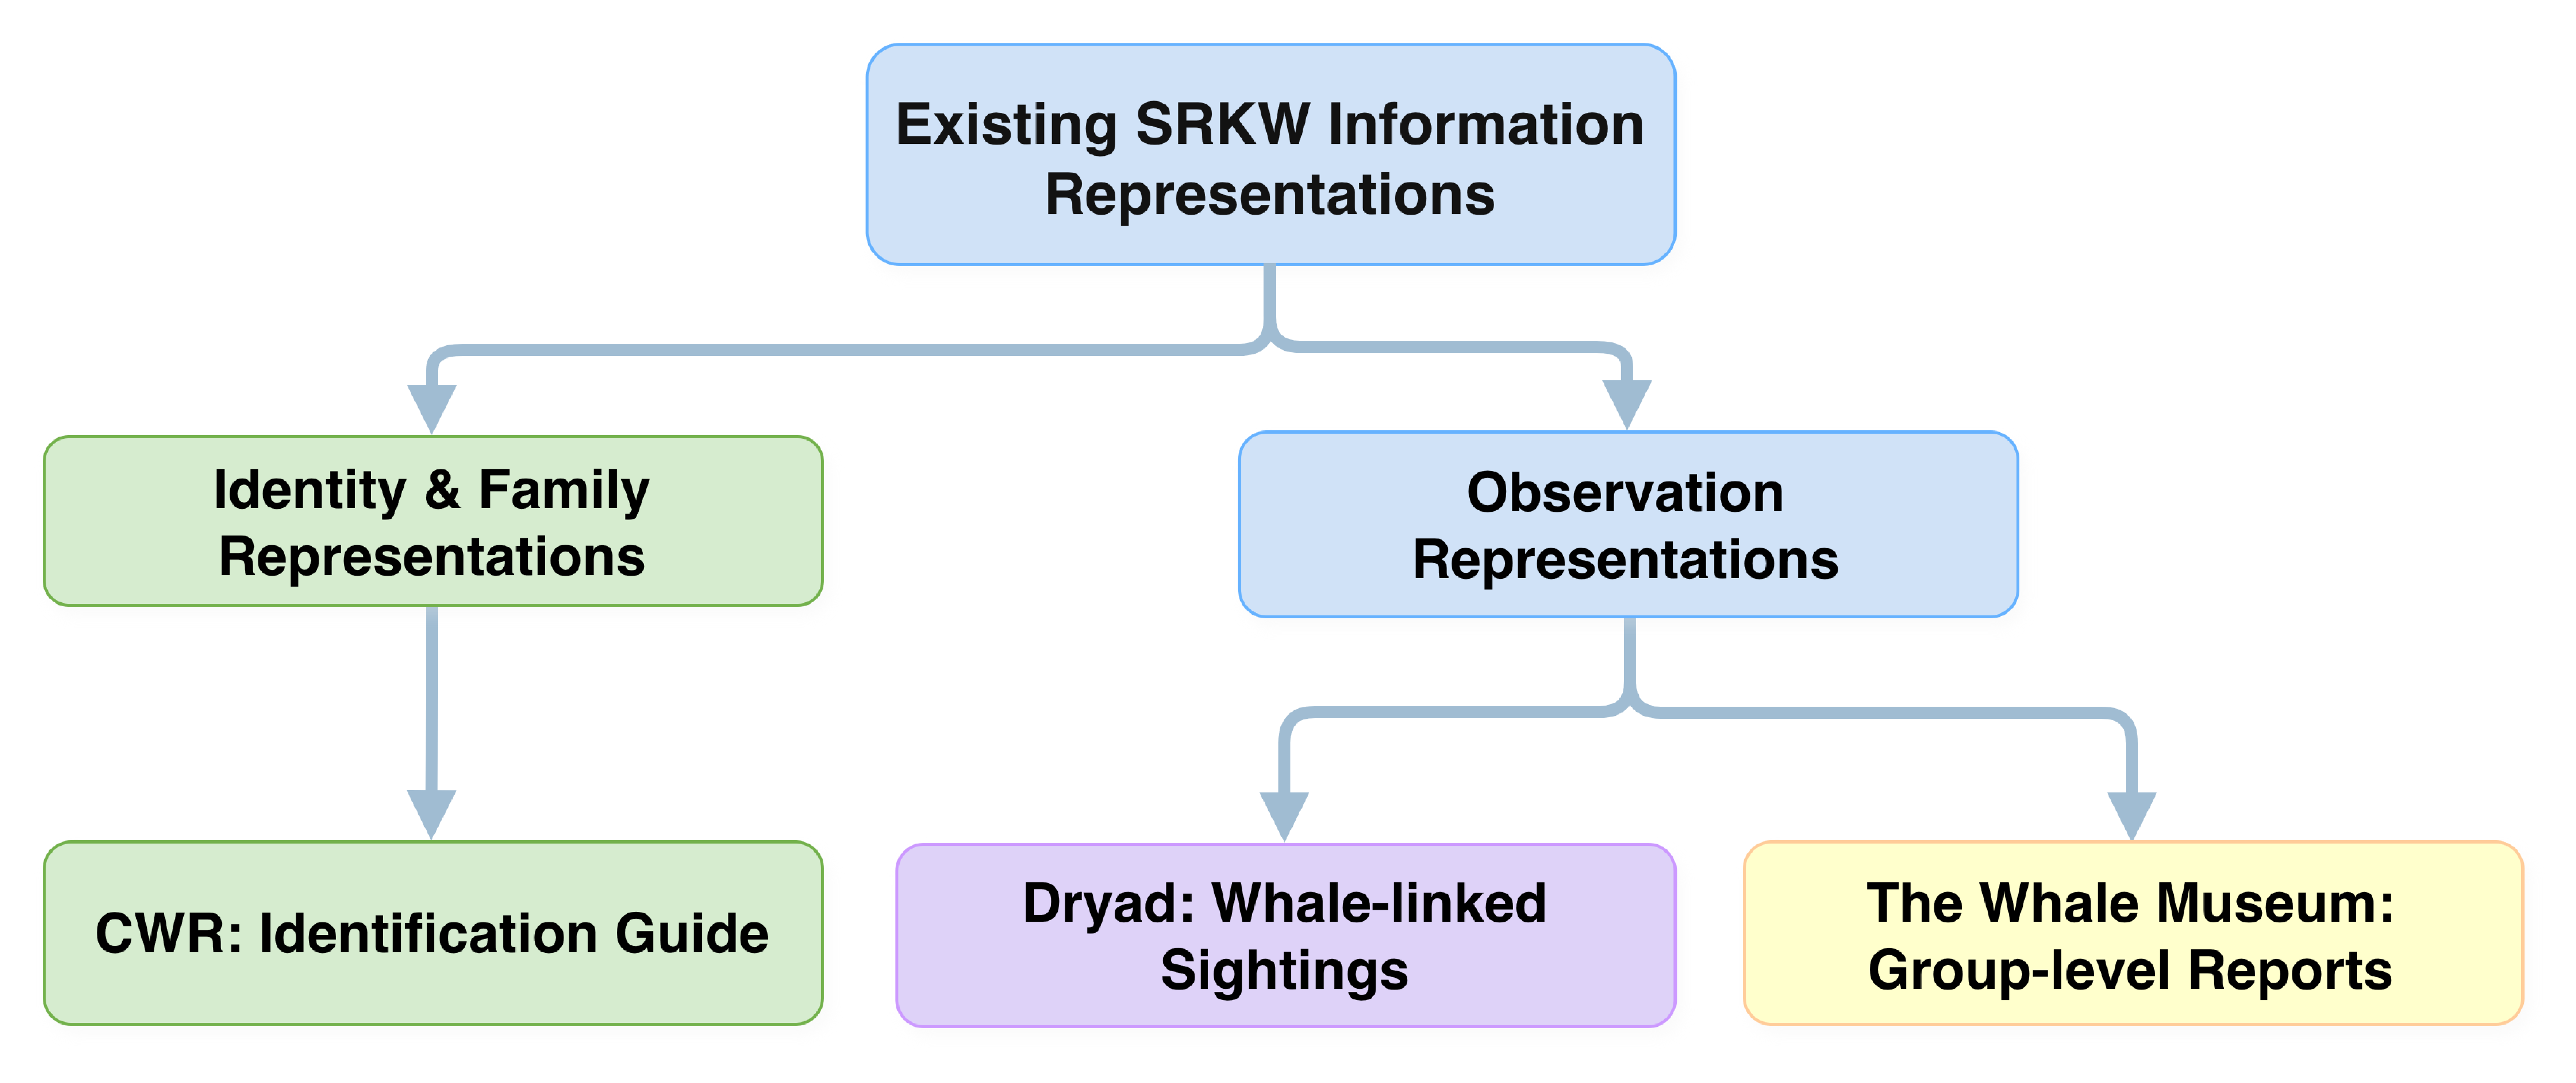
\includegraphics[width=\columnwidth]{Hierarchy.pdf}
    \caption{Categories of existing SRKW information representations reviewed for OrcaLink.}
    \label{fig:hierarchy}
\end{figure}

Identity and family representations, such as CWR's identification guides, organize individual whales by identity, pod, and matriline \cite{cwrOrcaID}. Observation representations are divided into whale-linked sightings and group-level reports. Dryad links whale records to sighting IDs, although some identifiers are inferred from group reports or are missing \cite{thompson2026dryad}. The supplied Whale Museum records describe reported groups, dates, and locations without individual whale IDs \cite{whalemuseum_dataset}. These categories highlight differences in purpose and detail that OrcaLink needs to preserve when combining the records.

\section{Comparative Analysis}

Table~\ref{tab:source-comparison} summarizes the main differences among the reviewed sources.

CWR's public records help describe individual whales and their family groups. Photo-identification allows the same whale to be recognized across encounters, while identification guides organize whales by pods and matrilines \cite{cwrOrcaID}. These records are useful for connecting identity and family information in OrcaLink. However, family membership alone does not tell us whether two whales were observed together in a particular encounter. Therefore, family relationships and recorded co-sightings need to be kept separate. Our comparison is currently limited to CWR's public records because the additional encounter data requested are still pending.

The Dryad dataset links whale records to observations through sighting IDs. Records with the same sighting ID represent whales counted together in one observation, which can support recorded co-sighting queries. However, some whale IDs were assigned based on reports of a whole pod or matriline rather than individual identification. Some observations also have missing IDs, so the presence of an ID cannot always be treated as an individually confirmed sighting. The lifespan file provides demographic information but does not include mother--offspring relationships. The timestamps and coordinates were also shifted, making matching with other sources more difficult \cite{thompson2026dryad}.

The Whale Museum dataset focuses on historical sighting reports. The Museum gathers reports and works to confirm sightings before entering them into its database \cite{whaleHotline}. The records provided for our project describe reported groups rather than individual whale IDs. They can help answer questions about when and where a group was reported, but cannot directly show which individual whales were together. The group labels also vary in detail. A named pod provides more identification information than a general label such as ``Orcas'' \cite{whalemuseum_dataset}.

Each source contributes different information: CWR describes identity and family structure, Dryad links whale records to observations, and the Whale Museum records reported group presence. OrcaLink must preserve each record's source and identification basis. Group reports do not confirm that every member was individually identified, and recorded co-sightings do not by themselves establish a close social relationship.

\section{Draft ER Model}

Figure~\ref{fig:erd} presents OrcaLink's draft ER model. Individual observations and group observations are separated so that a reported pod does not automatically identify every member. Individual observations retain identification status and basis, while data source records indicate whether timestamps or coordinates were shifted. Kinship is represented separately from associations. Association type, method, score, and time window distinguish recorded co-sightings from potential association candidates, with supporting sightings linked where available. These decisions address the differences identified in the comparison while preserving the evidence behind each connection.

\bibliographystyle{ACM-Reference-Format}
\bibliography{References}
\clearpage

\begin{figure*}[p]
    \centering
    \includegraphics[
        width=\textwidth,
        height=0.9\textheight,
        keepaspectratio
    ]{ERD.pdf}
    \caption{Draft entity--relationship model for OrcaLink.}
    \label{fig:erd}
\end{figure*}

\clearpage

\end{document}


\endinput
%%
%% End of file `sigconf.tex'.